\section{Ladningssensor}
\begin{figure}[H]
	\centering
    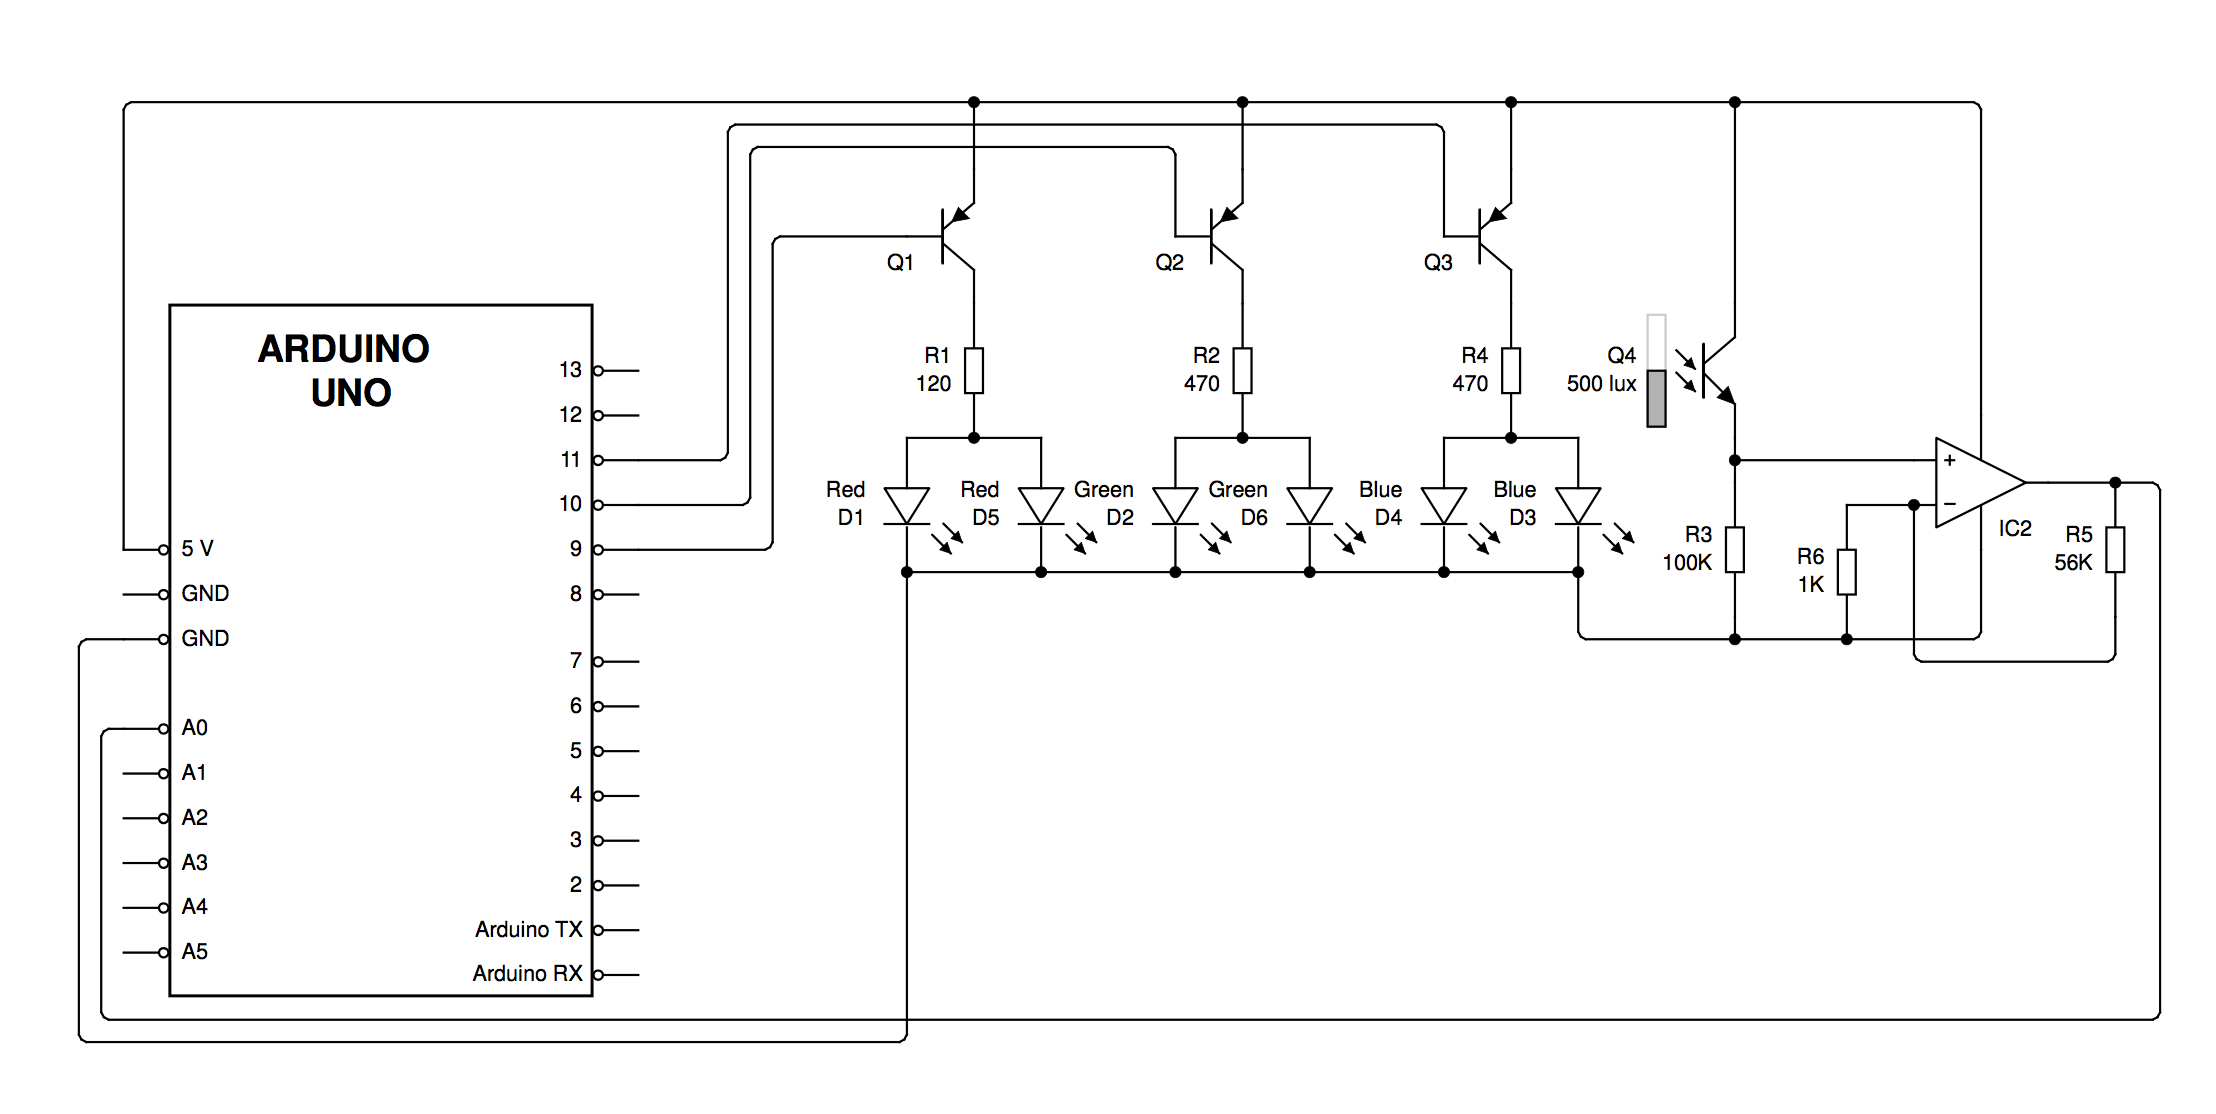
\includegraphics[width=\textwidth]{figures/CIRCUITS/farvesensorFinal.png}
	\caption{Et billede af kredsløbet for ladningssensor kredsen.}
	\label{fig:ladningsensor}
\end{figure}

\subsection{Komponenter}
\subsubsection{OP Amp - MCP601}
\begin{figure}[H]
	\centering
    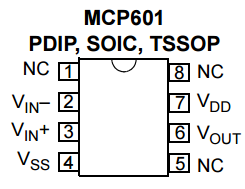
\includegraphics[width=7cm]{figures/komponenter/OPAMP}
	\caption{Bendiagram af MCP601}
	Se databladet i kilde \cite{kompOPAMP}.
\end{figure}
Vi benytter en OP Amp, til at forstærke signalet som vi modtager fra fotodioden, således at den bruger hele spændingsintervallet ($[\SI{0}{V};\SI{5}{V}]$) som Arduinoen kan måle i. Der er beskrevet mere om OP Amps i teoriafsnittet \ref{sec:OPAMP}.
\subsubsection{BPW21 - Fotodiode}
\begin{figure}[H]
	\centering
    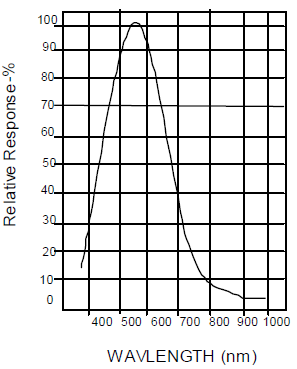
\includegraphics[height=10cm]{figures/komponenter/photosensor}
	\caption{Normal speltral respons angivet i procent}
	Se databladet i kilde \cite{kompPhoto}.
\end{figure}
BPW21 er en fotodiode, som betyder at det er en diode som omdanner lys til elektrisk strøm. \todo{skriv teori om BPW21}

\subsubsection{LED - RGB WHITE DIFFUSED LENS COMMON CATHODE}
\begin{figure}[H]
	\centering
    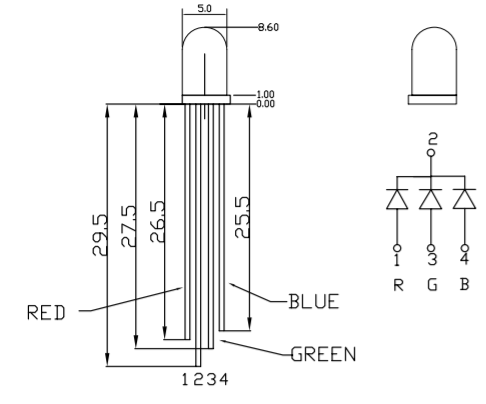
\includegraphics[height=7cm]{figures/komponenter/LED2}
	\caption{Diagram af LED'en}
	Se databladet i kilde \cite{kompRGBLED}.
\end{figure}
\begin{figure}[H]
	\centering
    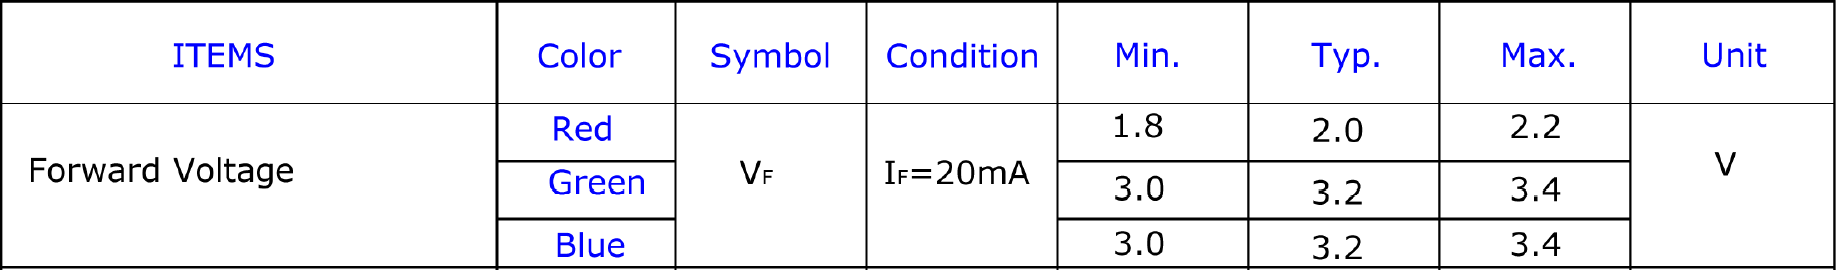
\includegraphics[width=\textwidth]{figures/komponenter/LED}
	\caption{Spændingsfaldet over de forskellige LED'er}
	Se databladet i kilde \cite{kompRGBLED}.
\end{figure}
Vi benytter en LED som kan lyse i 3 forskellige farver, rød, grøn og blå. Vi benyttede en LED med en fælles katode. Dette betyder at vi kan koble LED'ens katode til jord, også styre spændingen sat på hver af deres anoder. For ikke at trække for meget strøm fra arduinoen, benytter vi en PNP transistor som kontakt til LED'erne.

\subsubsection{PNP transistor}
\todo{Skriv om PNP transistor}

\subsubsection{Arduino}
Se afsnit \ref{sec:arduino} 

\subsection{Teori}
\subsubsection{OP Amp}\label{sec:OPAMP}
%%---------- indsæt billede---------------------------------%

En operationsforstærker (OP Amp) er en type forstærker der tager imod to inputs, inverting input voltage ($V_{in-}$) og non-inverting input voltage ($V_{in+}$). Outputtet fra en operationsforstærker  ($V_{out}$), kan beskrives med formlen
\begin{align}
V_{out}&=A(V_{in+}-V_{in-})\quad,\quad V^- \leq V_{out}\leq V^+ 
\end{align}
Her er $A$ den elektriske gain af operationsforstærkeren. $A$ er som reel omkring $10^5$ til $10^6$, men man anser den som at gå imod uendelig. Vi benyttede os af en non-inverting amplifier. 
\begin{figure}[H]
	\centering
    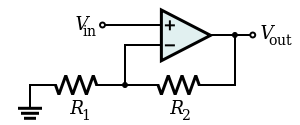
\includegraphics[width=\textwidth]{figures/komponenter/NonInvAmp}
	\caption{El diagram for non-inverting amplifier}
	\label{fig:noninvamp}	
\end{figure}
Som man kan se ud fra el diagrammet \ref{fig:noninvamp}, er der en spændingsdeler imellem $V_{out}$ og $V_{in-}$. Vi ved at for en spændingsfordeler gælder der
\begin{align}
U_{out}&=U\cdot \frac{R_2}{R_1+R_2}
\end{align}
Hvor at $U_{out}$ er spændingen over $R_2$ og $U$ er spændingen over $R_1$ og $R_2$.
Dette betyder at
\begin{align}
V_{in-}&=V_{out}\cdot \frac{R_2}{R_1+R_2}
\end{align}
Hvis vi indsætter dette i vores udtryk for $V_out$ gælder der
\begin{align}
V_{out}&=A(V_{in+}-V_{in-})\quad,\quad V^- \leq V_{out}\leq V^+\\
V_{in-}&=V_{out}\cdot \frac{R_2}{R_1+R_2}\\
\rightarrow V_{out}&= A(V_{in+}-V_{out}\cdot \frac{R_2}{R_1+R_2})\\
\rightarrow V_{out}+A\cdot V_{out}\cdot \frac{R_2}{R_1+R_2}&=A\cdot V_{in+}\\
\rightarrow V_{out}(1+A\cdot \frac{R_2}{R_1+R_2})&=A\cdot V_{in+}\\
\rightarrow V_{out}&=\frac{A\cdot V_{in+}}{1+A\cdot \frac{R_2}{R_1+R_2}}\\
\end{align}
Da $A$ er et meget højt tal, så kan $1$ i nævneren negligeres.
\begin{align}
V_{out}&=\frac{A\cdot V_{in+}}{A\cdot \frac{R_2}{R_1+R_2}}\\
&=\frac{V_{in+}}{\frac{R_2}{R_1+R_2}}\\
V_{out}&=V_{in+}\cdot(\frac{R_1}{R_2}+1)\\
\rightarrow \frac{V_{out}}{V_{in+}}&=\frac{R_1}{R_2}+1
\end{align}
Dette udtryk kan vi benytte til at beregne forstærkningen af vores non-inverting amplifier.
(Kilde: Teknik A - OP-amp DC-kobling (teori udleveret af læreren uden yderligere kildeangivelse))
\subsubsection{Analog input til registrering af farve}
Arduinoens analog input er beskrevet i afsnit \ref{sec:ard:analog}. Vi benytter denne funktion til at få outputtet fra vores farvesensor ind i arduinoen.
\subsection{Beregninger}
\subsubsection{Modstanden af LED}
Ifølge \cite{kompLED} gælder det for LED'en at dens typiske spænding for den blå og grønne LED
\[
	V_{GB typisk} = \SI{3.2}{V}
\]
Og for den røde 
\[
	V_{R typisk} = \SI{2}{V}
\]
Og kan klare en strømstyrke på
\[
	I = \SI{20d-3}{A} 
\]
Ud fra ohms lov må det betyde at hvis indgangsspændingen er på $\SI{5}{V}$, at modstanden til de enkelte LEDer skal være
\begin{align}
	R&= \frac{U}{I}\\
	R_{RLED} &= \frac{\SI{5}{V}-\SI{2}{V}}{\SI{2.0d-2}{A}} = \SI{150}{\ohm}\\
	R_{GLED} &= \frac{\SI{5}{V}-\SI{3.2}{V}}{\SI{2.0d-2}{A}} = \SI{90}{\ohm}\\
	R_{BLED} &= \frac{\SI{5}{V}-\SI{3.2}{V}}{\SI{2.0d-2}{A}} = \SI{90}{\ohm}\\
\end{align}
Ud fra dette valgte vi at benytte modstandene 
\begin{align}
	R_{RLED} &= \SI{180}{\ohm}\\
	R_{GLED} &= \SI{100}{\ohm}\\
	R_{BLED} &= \SI{100}{\ohm}\\
\end{align}
Det vidste sig dog at en LED ikke lyste nok op, og derfor satte vi en ekstra parallelt med den anden som vist på kredsløbstegningen. Dette betød at vi skulle beregne vores modstande igen. For en parallelforbindelse gælder
\begin{align}
\frac{1}{R_{tot}}&=\frac{1}{R_1}+\frac{1}{R_2}+...+\frac{1}{R_n}
\end{align}
hvor at der er $n$ parallelle modstande, som ønskes at erstattes med en samlet modstand $R_{tot}$. Da hver af de parallelle modstande, var de modstanden beregnet før, må den nye samlede modstand for hver farve være
\begin{align}
R_{R-tot}&=\frac{1}{\frac{1}{R_{RLED}}+\frac{1}{R_{RLED}}}\\
&=\frac{1}{\frac{1}{\SI{180}{\ohm}}+\frac{1}{\SI{180}{\ohm}}}\\
&=\SI{90}{\ohm}\\
R_{G-tot}&=\frac{1}{\frac{1}{R_{GLED}}+\frac{1}{R_{GLED}}}\\
&=\frac{1}{\frac{1}{\SI{100}{\ohm}}+\frac{1}{\SI{100}{\ohm}}}\\
&=\SI{50}{\ohm}\\
R_{B-tot}&=\frac{1}{\frac{1}{R_{BLED}}+\frac{1}{R_{BLED}}}\\
&=\frac{1}{\frac{1}{\SI{100}{\ohm}}+\frac{1}{\SI{100}{\ohm}}}\\
&=\SI{50}{\ohm}
\end{align}
Da vi havde beregnet de minimum modstande vi kunne bruge, prøvede vi os frem for at finde modstande, så hver LED lyste lige stærkt. Vi kom frem til disse modstande
\begin{align}
	R_{R-tot} &= \SI{120}{\ohm}\\
	R_{G-tot} &= \SI{470}{\ohm}\\
	R_{B-tot} &= \SI{470}{\ohm}\\
\end{align}
Her blev der lavet en test, af indgangsspændingen til Arduinoen, når der blev lyst med forskellige farver, på materialer med forskellig farve. Testen kan findes i tabel \ref{tab:farveudenforstaerker}. Hvis man ser på tegning \ref{fig:ladningsensor}, er den spænding vi måler i testen, spændingsfaldet fra A0 til ground.

\subsubsection{OPAMP modstande} \label{subs:opampanalog}
Vi besluttede os for at benytte en OPAMP, da vores største signal fra test 1 (se \ref{tab:farveudenforstaerker}) var på $\SI{0.06}{V}$, hvis man ser bort fra når alle lyser. Da vores precision af analog inputtet på arduinoen er omkring $\SI{0.005}{V}$ (se \ref{sec:ard:analog}), er disse udsving for små til at med sikkerhed kunne identificere farver. Vi benytter derfor en OPAMP, så det er nemmere at identificere hvilken farve der bliver brugt.
% R_in = 1k
% R_f = 56k
Vi valgte at den maksimale indgangsspænding til OPAMPen er
\[
	V_{in+} = \SI{0.08}{V}
\]
Vi ønsker at dette skal være det maksimale som Arduinoen kan måle ($\SI{5}{V}$)
\[
	V_{out} \approx \SI{5}{V}
\]
Heraf er den ønskede forstærkning
\[
	A_{target} = \frac{V_{out}}{V_{in+}} = \frac{\SI{5}{V}}{\SI{0.08}{V}}=62.5
\]

Denne forstærkning er ret høj og vi benytter derfor en non-inverting amplifier.

Vi bestemmer en rimelig værdi til den ene modstand er
\begin{align}
	R_{2} = \SI{1000}{\ohm} \label{eq:RinFarveOpAmp}
\end{align}
Og udtrykket for forstærkningen er

\begin{align}
	A_{target} = 1+\frac{R_1}{R_2} \label{eq:AtargetFarveOpAmp}
\end{align}
Ved at isolerer $R_1$ i ligningerne \ref{eq:RinFarveOpAmp} og \ref{eq:AtargetFarveOpAmp} fås
\[
	R_1 = \SI{61.5d3}{\ohm}
\]
Da vi ikke har denne modstand direkte, vælger vi at benytte en $\SI{56d3}{\ohm}$ modstand i stedet. Hvilket giver os en reel forstærkning på
\[
	A_{reel} = 1 + \frac{\SI{56d3}{\ohm}}{\SI{1000}{\ohm}} = 57	
\]
Hvilket svarer til et outputsignal på
\[
	V_{out} = \SI{0.08}\cdot 57 = \SI{4.56}{V}
\]
Hvilket er tilnærmelsesvis hvad vi gerne vil have. Derefter kørte vi den samme test som før vi havde forstærket signalet. Resultaterne kan ses i tabel \ref{tab:farvemedforstaerker}.





**** NOTER ****
Men da vi satte tre modstande ændrede vi det til ***. 
% MISC LED
Skriv LED anode eller cathode og indsæt tegning 
Simon → Farvesensor
Skriv om bestemmelse af modstande til LED
Start ->
G=100
B=100
R=180

Ændring ->
R=120
G=470
B=470

Skriv om arduino precision (10 bit)-> grunden til brug af opamps

Skriv om opAMP


Nævn af billederne i bilag (grøn blå) blev taget før at afstanden blev ændret fra 6 cm til 3cm.
(afstand 2 cm, mørklagt kasse)
% \usepackage[normalem]{ulem}
% \useunder{\uline}{\ul}{}

*************
\subsection{Test}
Vores teste foregik i en mørklagt kasse, hvor afstanden mellem sensoren og objektet var $\SI{2}{cm}$. Vi testede med 5 forskellige farver: hvid, rød, grøn, blå og gul. Vi kom frem til, ud fra vores test, at vores farvesensor efter forstærkning er tilstrækkelig til at kunne adskille farverne, hvid, rød, grøn og blå. Vi mener også dette lever op til vores krav for ladningssensoren, da vi så kan have 4 indstillinger, som vi mener er tilstrækkelig.


\begin{table}[H]
\centering
\caption{Signaler uden forstærkning} \label{tab:farveudenforstaerker}
\label{my-label}
\begin{tabular}{l|lllll}
\hline \hline
     & Alle{[\si{V}]} & Intet {[\si{V}]} & Rød{[\si{V}]} & Grøn{[\si{V}]} & Blå{[\si{V}]} \\
     \hline
Sort & 0.03        & 0.01          & 0.01       & 0.02        & 0.02       \\
Hvid & 0.12        & 0.01          & 0.02       & 0.06        & 0.06       \\
Rød  & 0.03        & 0.01          & 0.02       & 0.01        & 0.02       \\
Blå  & 0.05        & 0.01          & 0.01       & 0.02        & 0.03       \\
Gul  & 0.06        & 0.01          & 0.02       & 0.04        & 0.02       \\
Grøn & 0.04        & 0.01          & 0.01       & 0.03        & 0.02 \\[1ex]
\hline     
\end{tabular}
\end{table}
% Please add the following required packages to your document preamble:
% \usepackage[normalem]{ulem}
% \useunder{\uline}{\ul}{}
\begin{table}[H]
\centering
\caption{Signaler med forstærkning} \label{tab:farvemedforstaerker}
\begin{tabular}{l|lllll}
\hline\hline
     & Alle{[\si{V}]} & Intet {[\si{V}]} & Rød{[\si{V}]} & Grøn{[\si{V}]} & Blå{[\si{V}]} \\
     \hline
Sort & 0.47        & 0.05          & 0.08       & 0.23        & 0.25       \\
Hvid & 4.8         & 0.04          & 0.77       & 4.04        & 4.38       \\
Rød  & 1.03        & 0.06          & 0.53       & 0.29        & 0.28       \\
Blå  & 2.72        & 0.06          & 0.06       & 0.77        & 1.95       \\
Gul  & 3.8         & 0.06          & 0.75       & 2.42        & 0.75       \\
Grøn & 0.9         & 0.05          & 0.06       & 0.49        & 0.4 \\[1ex]
\hline
\end{tabular}
\end{table}

